% !TeX spellcheck = en_US
\section{Running experiment}\label{section:experiment-running}

In this chapter we will provide instructions for running experiment.

Before running experiment, learning data file (test data file is optional) should be created See \hyperref[section:isf-table]{Isf edition section}. It is recommended to fill all fields in active attributes. Condition attributes with empty values cannot be used in experiment, so experiment doesn't start with such values.

Also experiment properties should be configured. See \hyperref[section:properties]{Properties section}. All fields in properties should be set, either explicitly or by default values.

Experiment can be run from properties form. To do this, press ''Run Experiment'' button on top of properties form. After this isf table and experiment properties will be validated. If RUDE finds any misconfiguration error, it will display it on modal window and experiment doesn't start. If you provided multiple information sources (ranking, pairs or decision attribute), you will be asked to choose one of them.

\begin{figure*}[!ht] 
	\centering
	\makebox[\textwidth]{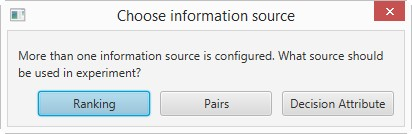
\includegraphics[width=.4\paperwidth]{raw/experiment-run-source}}
	\caption{Choose information source dialog}
\end{figure*}

Before experiment start, all properties will be logged (chosen properties and default ones for empty fields). When experiment finishes, all result files will be saved. In case of any errors, logs will be written to logs tab. Workspace tree will be automatically refreshed. If file names were not configured, they names will be calculated basing on learning and test data file name. The suffix partialPCT in some files is used to indicate that we deal with a “partial” PCT.

\vfill\newpage